\documentclass[final,t, mathserif]{beamer}
\mode<presentation>
{
\usetheme{I6dv}
%  \usetheme{I6pd}
%  \usetheme{I6pd2}
}
% additional settings
\setbeamerfont{itemize}{size=\normalsize}
\setbeamerfont{itemize/enumerate body}{size=\normalsize}
\setbeamerfont{itemize/enumerate subbody}{size=\normalsize}

% additional packages
\usepackage{times}
\usepackage{amsmath,amsthm, amssymb, latexsym}
\usepackage{graphicx, amssymb, listings}
%\usepackage[active]{srcltx}
%\usepackage[all,xdvi]{xy}
%\usepackage{showlabels}
\usepackage[alphabetic,y2k,lite]{amsrefs}

%%%%%%%%%%%%%%%%%% Tikz %%%%%%%%%
\usepackage{tikz}
\usetikzlibrary{arrows,backgrounds}
\usetikzlibrary{shapes.geometric}
\usetikzlibrary{calc}
\usetikzlibrary{scopes}
\usetikzlibrary{decorations.markings}
%\usepackage[labelformat=empty]{caption}

\tikzset{
every picture/.style={line width=0.8pt, >=stealth,
                       baseline=-3pt,label distance=-3pt},
%%%%%%%%%%  Node styles
dotnode/.style={fill=black,circle,minimum size=2.5pt, inner sep=1pt, outer
sep=0},
morphism/.style={circle,draw,thin, inner sep=1pt, minimum size=15pt,
                 scale=0.8},
small_morphism/.style={circle,draw,thin,inner sep=1pt,
                       minimum size=10pt, scale=0.8},
coupon/.style={draw,thin, inner sep=1pt, minimum size=18pt,scale=0.8},
%%%% different line styles:
regular/.style={densely dashed},
edge/.style={thick, dashed, draw=blue, text=black},
boundary/.style={thick,  draw=blue, text=black},
overline/.style={preaction={draw,line width=2mm,white,-}},
drinfeld center/.style={>=stealth,green!60!black, double
distance=1pt,text=black},
%%%%%%% Fill styles %%%%%%%%%%%%%%%
cell/.style={fill=black!10},
subgraph/.style={fill=black!30},
%%%%%%% Mid-path arrows
midarrow/.style={postaction={decorate},
                 decoration={
                    markings,% switch on markings
                    mark=at position #1 with {\arrow{>}},
                 }},
midarrow/.default=0.5
}
%%%%%%%%%%%%%%%%%%%%%%%%%%%%%%%%%%%%%%%%

\newcommand{\ph}{\varphi}
\renewcommand{\Im}{\mathrm{Im}}

\newcommand{\ee}{\mathbf{e}}
\DeclareMathOperator{\Obj}{Obj}
\DeclareMathOperator{\FPdim}{FPdim}
\DeclareMathOperator{\Hom}{Hom}
\DeclareMathOperator{\ev}{ev}
\DeclareMathOperator{\coev}{coev}
\DeclareMathOperator{\id}{id}
\DeclareMathOperator{\End}{End}
\DeclareMathOperator{\MCG}{MCG}
\DeclareMathOperator{\Homeo}{Homeo}
\DeclareMathOperator{\Vect}{Vect}
\DeclareMathOperator{\Mod}{Mod}
\DeclareMathOperator{\PGL}{PGL}

%\newtheorem{prop}[theorem]{Proposition}
%\newtheorem{conj}[theorem]{Conjecture}


\newcommand{\img}[1]{
\vfill
\centering
\includegraphics[width=\textwidth,height=0.8\textheight,keepaspectratio]{#1}
\vfill} 

%\usepackage{xy}

\usepackage{exscale}
%\boldmath
\usepackage{booktabs, array}
%\usepackage{rotating} %sideways environment
\usepackage[english]{babel}
\usepackage[latin1]{inputenc}
\usepackage[orientation=landscape,size=custom,width=120,height=90,scale=1.65]{beamerposter}
\listfiles
%\graphicspath{{figures/}}
% Display a grid to help align images
%\beamertemplategridbackground[1cm]



\title{\huge }
\author{Paul Gustafson}
\institute{Texas A\&M University}

% abbreviations
\usepackage{xspace}
\makeatletter
\DeclareRobustCommand\onedot{\futurelet\@let@token\@onedot}
\def\@onedot{\ifx\@let@token.\else.\null\fi\xspace}
\def\eg{{e.g}\onedot} \def\Eg{{E.g}\onedot}
\def\ie{{i.e}\onedot} \def\Ie{{I.e}\onedot}
\def\cf{{c.f}\onedot} \def\Cf{{C.f}\onedot}
\def\etc{{etc}\onedot}
\def\vs{{vs}\onedot}
\def\wrt{w.r.t\onedot}
\def\dof{d.o.f\onedot}
\def\etal{{et al}\onedot}
\makeatother

\newcommand{\arXiv}[1]{\url{http://arxiv.org/abs/#1}}
\newcommand{\doi}[1]{\href{http://dx.doi.org/#1}{{\tt DOI:#1}}}
\newcommand{\euclid}[1]{\href{http://projecteuclid.org/getRecord?id=#1}{{\tt #1}}}
\newcommand{\mathscinet}[1]{\href{http://www.ams.org/mathscinet-getitem?mr=#1}{\tt #1}}
\newcommand{\googlebooks}[1]{(preview at \href{http://books.google.com/books?id=#1}{google books})}

%%%%%%%%%%%%%%%%%%%%%%%%%%%%%%%%%%%%%%%%%%%%%%%%%%%%%%%%%%%%%%%%%%%%%%%%%%%%%%%%%%%%%%%%%%%%%%%%%%%%%%%%%%%%
\theoremstyle{plain}
\newtheorem{thm}{Theorem}[section]
\newtheorem{cor}[thm]{Corollary}
\newtheorem{conjec}[thm]{Conjecture}
\newtheorem{lem}[thm]{Lemma}
\newtheorem{prop}[thm]{Proposition}
\newtheorem{quest}[thm]{Question}
\theoremstyle{definition}
\newtheorem{defn}[thm]{Definition}
\newtheorem{prob}[thm]{Problem}
\newtheorem{nota}[thm]{Notation}
\newtheorem{notes}[thm]{Notes}
\newtheorem{exs}[thm]{Examples}
\newtheorem{ex}[thm]{Example}
\newtheorem{rem}[thm]{Remark}
\newtheorem{rems}[thm]{Remarks} 
\newtheorem{alg}[thm]{Algorithm} 


% Operators %%%%%%%%%%%%%%%%%%%%%%%%%%%%%%%%%
\DeclareMathOperator{\coker}{coker}
\DeclareMathOperator{\capind}{capind}
\DeclareMathOperator{\caps}{caps}
\DeclareMathOperator{\cupind}{cupind}
\DeclareMathOperator{\cups}{cups}
%\DeclareMathOperator{\id}{id}
\DeclareMathOperator{\im}{im}
\DeclareMathOperator{\ind}{ind}
%\DeclareMathOperator{\Hom}{Hom}
\DeclareMathOperator{\Ob}{Ob}
\DeclareMathOperator{\rel}{rel}
\DeclareMathOperator{\tr}{tr}
\DeclareMathOperator{\sh}{sh}
\DeclareMathOperator{\spann}{span}
% Math %%%%%%%%%%%%%%%%%%%%%%%%%%%%%%%%%
\newcommand{\D}{\displaystyle}
\newcommand{\comment}[1]{}
\newcommand{\hs}{\hspace{.07in}}
\newcommand{\hsp}[1]{\hs\text{#1}\hs}
\newcommand{\be}{\begin{enumerate}}
%\newcommand{\ee}{\end{enumerate}}
\newcommand{\itm}[1]{\item[\underline{\ensuremath{#1}:}]} 
\newcommand{\itt}[1]{\item[\underline{\text{#1}:}]} 
\newcommand{\N}{\mathbb{N}}
\newcommand{\R}{\mathbb{R}}
\newcommand{\PP}{\mathbb{P}}
\newcommand{\C}{\mathbb{C}}
\newcommand{\F}{\mathbb{F}}
\newcommand{\Z}{\mathbb{Z}} 
\newcommand{\W}{\mathcal{W}} 
\newcommand{\T}{\mathcal{T}} 
\newcommand{\I}{\infty} 
\newcommand{\set}[2]{\left\{#1 \big| #2\right\}}
\newcommand{\SET}[2]{\left\{#1 \bigg| #2\right\}}
\newcommand{\thh}{^{\text{th}}}
\newcommand{\stt}{^{\text{st}}}
\newcommand{\A}{\mathcal{A}}
\newcommand{\B}{\mathcal{B}}
\newcommand{\E}{\mathcal{E}}
\newcommand{\V}{\mathcal{V}}
% Categories %%%%%%%%%%%%%%%%%%%%%%%%%%%%%%%%%
\newcommand{\Atl}{{\sf{Atl}}}
\newcommand{\AAA}{{\sf{A}}}
\newcommand{\BB}{{\sf{B}}}
\newcommand{\DD}{{\sf{D}}}
\newcommand{\TT}{{\sf{T}}}
\newcommand{\PO}{{\sf{PO}}}
\newcommand{\Q}{{\mathfrak{Q}}}
\newcommand{\el}{{\mathfrak{L}}}
\newcommand{\CC}{{\mathfrak{C}}}
\newcommand{\QQ}{{\sf{Q}}}
\newcommand{\cAtl}{{\sf{cAtl}}} 
\newcommand{\sAtl}{{\sf{sAtl}}}
\newcommand{\ssAtl}{{\sf{ssAtl}}} 
\newcommand{\aD}{{\sf{a}\Delta}}
\newcommand{\tlD}{{\sf{tl}\Delta}}
\newcommand{\ccD}{{\sf{c}\Delta}}
\newcommand{\sD}{{\sf{s}\Delta}}
\newcommand{\ssD}{{\sf{ss}\Delta}}
\newcommand{\TL}{{\sf{TL}}}
\newcommand{\sTL}{{\sf{sTL}}}
\newcommand{\ssTL}{{\sf{ssTL}}}
\newcommand{\aTL}{{\sf{aTL}}}
\newcommand{\Fun}{\sf{Fun}}
%\newcommand{\Vect}{\sf{Vect}}
\newcommand{\Cat}{\sf{Cat}}
\newcommand{\Set}{\sf{Set}}
\newcommand{\Hilb}{{\sf{Hilb}}}
\newcommand{\RMod}[1]{{\sb{#1}\sf{Mod}}}
\newcommand{\ModR}[1]{{\sf{Mod}_#1}} 
\newcommand{\op}{^{\sf{op}}}   


%%%%%%%%%%%%%%%%%%%%%%%%%%%%%%%%%%%%%%%%%%%%%%%%%%%%%%%%%%%%%%%%%%%%%%%%%%%%%%%%%%%%%%%%%%%%%%%%%%
\begin{document}
\tikzstyle{shaded}=[fill=red!10!blue!20!gray!30!white]
\tikzstyle{shaded line}=[double=red!10!blue!20!gray!30!white, double distance=1.5mm, draw=black]
\tikzstyle{unshaded}=[fill=white]
\tikzstyle{unshaded line}=[double=white, double distance=1.5mm, draw=black]
\tikzstyle{Tbox}=[circle, draw, thick, fill=white, opaque,]
\tikzstyle{empty box}=[circle, draw, thick, fill=white, opaque, inner sep=2mm]
\tikzstyle{background rectangle}= [fill=red!10!blue!20!gray!40!white,rounded corners=2mm] 
\tikzstyle{on}=[very thick, red!50!blue!50!black]
\tikzstyle{off}=[gray]

%These are for resizing a family of drawings at the same time
\tikzstyle{traces}=[scale=.2, inner sep=1mm]
\tikzstyle{quadratic}=[scale=.4, inner sep=1mm, baseline]
\tikzstyle{annular}=[scale=.7, inner sep=1mm, baseline]
\tikzstyle{rectangular}=[scale=.75, inner sep=1mm, baseline]
\tikzstyle{make triple edge size}= [scale=.4, inner sep=1mm,baseline] 
\tikzstyle{icosahedron network}=[scale=.3, inner sep=1mm, baseline]
\tikzstyle{ATLsix}=[scale=.25, baseline]
\tikzstyle{TL12}=[scale=.15,baseline]
\tikzstyle{PAdefn}=[scale=.7,baseline]
\tikzstyle{TLEG}=[scale=.5,baseline]
\begin{frame}{} 
  \begin{columns}[t]
    
\begin{column}{.3\linewidth}

%%%%%%%%%%%%%%%%%%%%%%%%%%%%%%%%%%%%%%%%%%%%%%%%%

  \begin{block}{Mapping class groups}

    \begin{itemize}
    
\item
   The mapping class group of a compact surface $\Sigma$, 
   $\MCG(\Sigma),$
   is the group of isotopy classes of orientation-preserving self-homeomorphisms of $\Sigma$ 
  \begin{itemize}
    \item $\MCG(\mathbf{D} \text{ with } n \text{ marked points}) = B_m$
    \item $\MCG(\mathbf{T}^2) = SL(2,\mathbb Z)$
  \end{itemize}
\end{itemize}
\end{block}

%%%%%%%%%%%%%%%%%%%%%%%%%%%%%%%%%%%%%%%%%%%%%%%%%


\begin{block}{Property F conjecture for mapping class groups (Rowell)}
The Turaev-Viro-Barrett-Westbury (TVBW) mapping class group representation associated to a compact surface $\Sigma$ and spherical fusion category $\mathcal A$ has finite image iff $\mathcal A$ is weakly integral.
\end{block}


\begin{block}{The spherical fusion category $\Vect^\omega_G$}
  Our case: $\Vect^\omega_G$, the category $G$-graded vector spaces with a twist
\begin{itemize} 
\item The associator $\alpha_{g,h,k}:(V_g \otimes V_h) \otimes V_k \to V_g \otimes (V_h \otimes V_k)$
            $$ \alpha_{g,h,k} = \omega(g,h,k)$$
\item The evaluator $\ev_g:V_g^* \otimes V_g \to 1$
  $$ ev_g = \omega(g^{-1},g,g^{-1})$$
\item The coevaluator $\coev_g:V_g \otimes V_g^* \to 1$
    $$\coev_g = 1$$
\item The pivotal structure $j_g:V_g^{**} \to V_g$
            $$ j_g = \omega(g^{-1},g,g^{-1})$$
\end{itemize}

\end{block}


\begin{block}{Related Work}
  \begin{itemize}
  \item All $\Vect_G^\omega$ braid group representations have finite images (Etingof--Rowell--Witherspoon)

  \item  If $\omega = 1$, every mapping class group representation of a closed surface with $\le 1$ marked point has finite image
(Fjelstad--Fuchs)

  \item Every $SL(2,\mathbf{Z})$ representation from any modular category has finite image (Ng--Schauenberg)
  \end{itemize}
\end{block}

\end{column}
\begin{column}{.3\linewidth}




\begin{block}{Main result}
The image of any $\Vect^\omega_G$ TVBW representation $\rho$ of a mapping class group of an orientable, compact surface $\Sigma$ with boundary is finite.
\\ \vspace{1cm}
Proof outline:
\begin{itemize}
  \item Describe a tractable presentation of  the representation space
  \item Find a good finite spanning set $S$ for the representation space
  \item Calculate the action of each Birman generator on $S$
  \item Show that the representation of each Birman generator lies in a quotient of a finite group of monomial matrices.  
\end{itemize}
\end{block}

\begin{block}{The TVBW space associated to a 2-manifold}
  \begin{itemize}
    \item 
        Kirillov: The TVBW representation space is canonically isomorphic to
        \[
        H := \frac{\mathbf{C}[\text{$\mathcal A$-colored graphs in $\Sigma$}] }
        {\text{local relations}}
       \]
  \end{itemize}

\end{block}

%% \begin{block}{Colored graphs in $\Sigma$}
%% \begin{itemize}
%% \item Let $\Gamma \subset \Sigma$ be an undirected finite graph embedded in $\Sigma$.

%%  \item Define $E^{or}$ to be the set of orientation edges of $\Gamma$, i.e. pairs $\ee=(e,\text{orientation of } e)$; for such an oriented edge $\ee$, we denote by $\bar{\ee}$ the edge with opposite orientation. 

%%  \item A {\em coloring} of $\Gamma$ is the
%% following data: 
%% \begin{itemize}
%%     \item Choice of an object $V(\ee)\in \Obj \mathcal A$ for every oriented edge  $\ee \in E^{or}$ so that $V(\bar{\ee})=V(\ee)^*$.
%%      \item Choice of a vector $\ph(v)\in \Hom_{\mathcal A}(1, V_1 \otimes \cdots \otimes V_n)$  for  every interior vertex $v$, where 
%%       $\ee_1, \dots, \ee_n$ are edges incident to $v$, taken in counterclockwise
%%       order and with outward orientation.
%% \end{itemize}
%% \end{itemize}
%% \end{block}


\begin{block}{Local relations}
\begin{itemize}
\item Isotopy of the graph embedding
\item Linearity in the vertex colorings
\end{itemize}

\begin{figure}[ht]
%%%%%%%%%%%%%%%%%%%%%%%%%%%%%%%%%%%%%%%%%%%%%%%%%%%%%%%
%%%%%%%%%%

\begin{tikzpicture}
\node[morphism] (ph) at (0,0) {$\ph$};
\node[morphism] (psi) at (1,0) {$\psi$};
\node at (-0.7,0.1) {$\vdots$};
\node at (1.7,0.1) {$\vdots$};
\draw[->] (ph)-- +(220:1cm) node[pos=1.0,below,scale=0.8]
{$V_n$};
\draw[->] (ph)-- +(140:1cm) node[pos=1.0,above,scale=0.8]
{$V_1$};
\draw[->] (psi)-- +(40:1cm) node[pos=1.0,above,scale=0.8]
{$W_m$};
\draw[->] (psi)-- +(-40:1cm) node[pos=1.0,below,scale=0.8]
{$W_1$};
\draw[->] (ph) -- (psi) node[pos=0.5,above,scale=0.8] {$X$};
\end{tikzpicture}
%%%%%%%%
=
%%%%%%%%
\begin{tikzpicture}
\node[ellipse, thin, scale=0.8, inner sep=1pt, draw] (ph) at (0,0)
             {$\ph\circ_{X}\psi$};
\node at (-0.8,0.1) {$\vdots$};
\node at (0.8,0.1) {$\vdots$};
\draw[->] (ph)-- +(220:1cm) node[pos=1.0,below,scale=0.8] {$V_n$};
\draw[->] (ph)-- +(140:1cm) node[pos=1.0,above,scale=0.8] {$V_1$};
\draw[->] (ph)-- +(40:1cm) node[pos=1.0,above,scale=0.8]  {$W_m$};
\draw[->] (ph)-- +(-40:1cm) node[pos=1.0,below,scale=0.8] {$W_1$};
\end{tikzpicture}
%%%%%%%%%
\\
%%%%%%%%%
\begin{tikzpicture}
\node[dotnode] (ph) at (0,0) {};
\node[dotnode] (psi) at (1.5,0) {};
\node at (-0.7,0.1) {$\vdots$};
\node at (2.2,0.1) {$\vdots$};
\draw[->] (ph)-- +(220:1cm) node[pos=1.0,below,scale=0.8] {$A_n$};
\draw[->] (ph)-- +(140:1cm) node[pos=1.0,above,scale=0.8] {$A_1$};
\draw[->] (psi)-- +(40:1cm) node[pos=1.0,above,scale=0.8] {$B_m$};
\draw[->] (psi)-- +(-40:1cm) node[pos=1.0,below,scale=0.8] {$B_1$};
\draw[out=45,in=135, midarrow] (ph) to (psi)
                node[above,xshift=-0.6cm, yshift=0.25cm, scale=0.8] {$V_k$};
\draw[ out=15,in=165, midarrow] (ph) to (psi);
\draw[ out=-15,in=195, midarrow] (ph) to (psi);
\draw[ out=-45,in=225, midarrow] (ph) to (psi) node[below, xshift=-0.6cm, yshift=-0.3cm, scale=0.8] {$V_1$};
\end{tikzpicture}
%%%%%%%%%%%
=
%%%%%%%%%%%
\begin{tikzpicture}
\node[dotnode] (ph) at (0,0) {};
\node[dotnode] (psi) at (1.5,0) {};
\node at (-0.7,0.1) {$\vdots$};
\node at (2.2,0.1) {$\vdots$};
\draw[->] (ph)-- +(220:1cm) node[pos=1.0,below,scale=0.8] {$A_n$};
\draw[->] (ph)-- +(140:1cm) node[pos=1.0,above,scale=0.8] {$A_1$};
\draw[->] (psi)-- +(40:1cm) node[pos=1.0,above,scale=0.8] {$B_m$};
\draw[->] (psi)-- +(-40:1cm) node[pos=1.0,below,scale=0.8] {$B_1$};
\draw[ ->] (ph) to (psi)
            node[above,xshift=-0.8cm,scale=0.8] {$V_1\otimes \dots\otimes V_k$};
\end{tikzpicture}
%%%%%%%
\qquad $k\ge 0$
\\
%%%%%%%
\begin{tikzpicture}
\node[ellipse, scale=0.8, inner sep=1pt, draw,thin] (ph) at (0,0)
{$\mathrm{coev}$};
\draw[->] (ph)-- +(180:1cm) node[pos=1.0,above,scale=0.8] {$V$};
\draw[->] (ph)-- +(0:1cm) node[pos=1.0,above,scale=0.8] {$V^*$};
\end{tikzpicture}
%%%%%%%%
=
%%%%%%%%
\begin{tikzpicture}
\draw[->] (2,0)-- (0,0) node[pos=0.5,above,scale=0.8] {$V$};
\end{tikzpicture}
%%%%%%%%%%%%%%%%%%%%%%%%%%
\caption{The remaining local relations.
        }\label{f:local_rels1}
\end{figure}

\end{block}

%% \begin{block}{Consequences of the local relations}

%% \begin{figure}[ht]
%% %%%%%%%%%%%%
%% \begin{tikzpicture}
%% \node[morphism] (ph) at (0,0) {$\ph$};
%% \node[morphism] (psi) at (1.5,0) {$\psi$};
%% \node at (-0.7,0.1) {$\vdots$};
%% \node at (2.2,0.1) {$\vdots$};
%% \draw[->] (ph)-- +(220:1cm) node[pos=1.0,below,scale=0.8] {$V_n$};
%% \draw[->] (ph)-- +(140:1cm) node[pos=1.0,above,scale=0.8] {$V_1$};
%% \draw[->] (psi)-- +(40:1cm) node[pos=1.0,above,scale=0.8] {$W_m$};
%% \draw[->] (psi)-- +(-40:1cm) node[pos=1.0,below,scale=0.8] {$W_1$};
%% \draw[->] (ph) -- (psi) node[pos=0.5,above,scale=0.8] {$X_1\oplus X_2$};
%% \end{tikzpicture}
%% %%%%%%%%%%%%
%% =
%% %%%%%%%%%%%%
%% \begin{tikzpicture}
%% \node[morphism] (ph) at (0,0) {$\ph_1$};
%% \node[morphism] (psi) at (1.5,0) {$\psi_1$};
%% \node at (-0.7,0.1) {$\vdots$};
%% \node at (2.2,0.1) {$\vdots$};
%% \draw[->] (ph)-- +(220:1cm) node[pos=1.0,below,scale=0.8]{$V_n$};
%% \draw[->] (ph)-- +(140:1cm) node[pos=1.0,above,scale=0.8]{$V_1$};
%% \draw[->] (psi)-- +(40:1cm) node[pos=1.0,above,scale=0.8]{$W_m$};
%% \draw[->] (psi)-- +(-40:1cm) node[pos=1.0,below,scale=0.8]{$W_1$};
%% \draw[->] (ph) -- (psi) node[pos=0.5,above,scale=0.8] {$X_1$};
%% \end{tikzpicture}
%% %%%%%%%%%%%%
%% +
%% %%%%%%%%%%%%
%% \begin{tikzpicture}
%% \node[morphism] (ph) at (0,0) {$\ph_2$};
%% \node[morphism] (psi) at (1.5,0) {$\psi_2$};
%% \node at (-0.7,0.1) {$\vdots$};
%% \node at (2.2,0.1) {$\vdots$};
%% \draw[->] (ph)-- +(220:1cm) node[pos=1.0,below,scale=0.8]{$V_n$};
%% \draw[->] (ph)-- +(140:1cm) node[pos=1.0,above,scale=0.8]{$V_1$};
%% \draw[->] (psi)-- +(40:1cm) node[pos=1.0,above,scale=0.8]{$W_m$};
%% \draw[->] (psi)-- +(-40:1cm) node[pos=1.0,below,scale=0.8]{$W_1$};
%% \draw[->] (ph) -- (psi) node[pos=0.5,above,scale=0.8] {$X_2$};
%% \end{tikzpicture}
%% %%%%%%%%%%%%


%% \caption{Additivity in edge colorings. Here $\ph_1,\ph_2$ are compositions
%% of $\ph$ with projector $X_1\oplus X_2\to X_1$ (respectively, 
%% $X_1\oplus X_2\to X_2$), and similarly for $\psi_1,\psi_2$.
%% }
%% \end{figure}

%% \begin{itemize}
%% \item Additivity in edge colorings
%% \end{itemize}

%%   \begin{theorem}[Kirillov, Reshitikhin--Turaev]
%%   A colored graph $\Gamma$ may be evaluated on any disk $D\subset \Sigma$, giving
%%   an equivalent colored graph $\Gamma'$ such that $\Gamma'$ is identical
%%   to $\Gamma$ outside of $D$, has the same colored edges crossing $\partial D$,
%%   and contains at most one colored vertex within $D$.
%%   \end{theorem}

%% \end{block}


\end{column}
\begin{column}{.3\linewidth}

\begin{block}{Spanning set for the representation space}
  %% By applying the local moves and the preceding theorem, any such representation space has a finite spanning set of ``simple'' colored graphs with a single vertex, loops for each of the standard generators of $\pi_1(\Sigma)$, and a leg from the vertex to each of the boundary components.  

\newdimen\R
\R=0.7cm
  
\begin{figure}
   \centering
    \begin{tikzpicture}[scale=3]    

      \draw (0:\R) \foreach \x in {45,90,...,359} {
                -- (\x:\R)
            } -- cycle;
      
                 
    \begin{scope}[very thick,decoration={
    markings,
    mark=at position 0.5 with {\arrow{>}}}
    ]  
      \draw[postaction={decorate}]  (0, 0) --  (22: {0.923879*\R}) node[pos=.5,sloped,above]{$g$};
      \draw[postaction={decorate}]  (0, 0) --  (67: {0.923879*\R}) node[pos=.5,above]{$h$};
      \draw[postaction={decorate}]  (112: {0.923879*\R}) -- (0, 0) node[pos=.5,above]{$g$};
      \draw[postaction={decorate}]  (157: {0.923879*\R}) -- (0, 0) node[pos=.5,sloped,above]{$h$};
      \draw[postaction={decorate}]  (0, 0) --  (202: {0.923879*\R}) node[pos=.5,sloped,above]{$k$};
      \draw[postaction={decorate}]  (0, 0) --  (247: {0.923879*\R}) node[pos=.5,sloped,above]{$l$};
      \draw[postaction={decorate}]  (292: {0.923879*\R}) -- (0, 0) node[pos=.5,sloped,above]{$k$};
      \draw[postaction={decorate}]  (337: {0.923879*\R}) -- (0, 0) node[pos=.5,sloped,above]{$l$};
    \end{scope}
    \end{tikzpicture}
%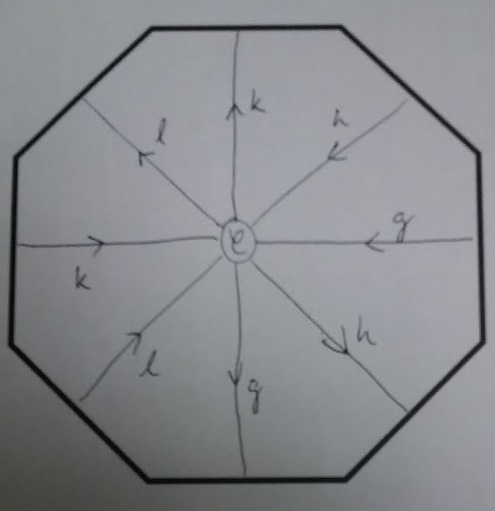
\includegraphics[width=0.5\textwidth]{basis.jpg}
\caption{Element of the spanning set for a genus 2 surface.  Here $[g,h][k,l] = 1$, and the vertex is labeled by a ``simple'' morphism (a $|G|$-th root of unity times a canonical morphism)}
\label{fig:span}
\end{figure}
\end{block}


\begin{block}{Applying the Birman generators to the spanning set}
\begin{itemize}
\item  The next step of the proof is to apply each Birman generator to each element of the spanning set.
\item  In each case, we relate the resulting colored graph to another element of the spanning set by means of local moves
\item  The local moves map simple colored graphs to simple colored graphs
\item Hence, the Birman generators preserve the finite spanning set.
\end{itemize}
\end{block}

%% \begin{block}{Applying the Birman generators to the spanning set}
%% \begin{prop}[G.]
%% Let $\Gamma$ be a simple colored graph embedded in a surface $\Sigma$.  Let $\Delta$ be the colored graph given by applying one of the three local moves in Figure \ref{f:local_rels1} to $\Gamma$.  Then
%% \begin{enumerate}
%% \item  each edge of $\Delta$ is labeled by $\delta_g$ for some $g \in G$, and
%% \item  there exists $\alpha \in \mu_{|G|}$ such that 
%% $$\Delta = \alpha \Delta' $$
%% in $H$, where $\Delta'$ is a simple colored graph given by replacing each vertex label in $\Delta$ with a simple morphism.
%% \end{enumerate}
%% \end{prop}
%% \end{block}
  
\begin{block}{First Dehn twist}
\img{t1}
\end{block}

\begin{block}{Second Dehn twist}
\img{t2}
\end{block}

\begin{block}{Braid generator}
\img{t3}
\end{block}

\begin{block}{Dragging a point}
\img{t4}
\end{block}



%% %%%%%%%%%%%%%%%%%%%%%%%%%%%%%%%%%%%%%%%%%%%%%%%%%

%% \begin{block}{References}
%% \scriptsize{
%% \bibliographystyle{amsalpha}
%% \bibliography{bibliography}
%% }
%% \end{block}

%% %%%%%%%%%%%%%%%%%%%%%%%%%%%%%%%%%%%%%%%%%%%%%%%%%

\end{column}
\end{columns}
\end{frame}
\end{document}
